% This Source Code Form is subject to the terms of the Mozilla Public
% License, v. 2.0. If a copy of the MPL was not distributed with this
% file, You can obtain one at http://mozilla.org/MPL/2.0/.
%
% Copyright (c) 2011-2019 ETH Zurich.

\documentclass[orivec]{llncs}

\usepackage{stmaryrd}
\usepackage{galois}
\usepackage{amssymb}
\usepackage{amsmath}
\usepackage{subfigure}
\usepackage{graphicx}
\usepackage{fancyvrb}
\usepackage{url}
\usepackage{wrapfig}

\urldef{\mailpietro}\path|{pietro.ferrara}@inf.ethz.ch|   
\urldef{\mailgiuliatino}\path|{costantini, cortesi}@dsi.unive.it|    
\newcommand{\keywords}[1]{\par\addvspace\baselineskip
\noindent\keywordname\enspace\ignorespaces#1}

\newbox\subfigbox
\makeatletter
\newenvironment{subfloat}
{\def\caption##1{\gdef\subcapsave{\relax##1}}%
\let\subcapsave=\@empty
\let\sf@oldlabel=\label
\def\label##1{\xdef\sublabsave{\noexpand\label{##1}}}%
\let\sublabsave\relax
\setbox\subfigbox\hbox
\bgroup}
{\egroup
\let\label=\sf@oldlabel
\subfigure[\subcapsave]{\box\subfigbox}}%
\makeatother

% This Source Code Form is subject to the terms of the Mozilla Public
% License, v. 2.0. If a copy of the MPL was not distributed with this
% file, You can obtain one at http://mozilla.org/MPL/2.0/.
%
% Copyright (c) 2011-2019 ETH Zurich.

\newcommand{\Sample}{\ensuremath{\mathsf{Sample}}}

\newcommand{\todo}[1]{\textbf{TODO:#1}}
%\newcommand{\todogiulia}[1]{\textbf{TODO GIULIA: #1}}
%\newcommand{\emphgiulia}[1]{\textbf{#1}}
%\newcommand{\emphgiulia}[1]{#1}
%\newcommand{\newpart}[1]{\hl{#1}}
\newcommand{\goodgap}{\hspace{1.536pt}}


\newcommand{\Java}{\ensuremath{\mathsf{Java}}}
\newcommand{\Scala}{\ensuremath{\mathsf{Scala}}}
\newcommand{\CSharp}{\ensuremath{\mathsf{C\#}}}
\newcommand{\FSharp}{\ensuremath{\mathsf{F\#}}}

\newcommand{\lfp}[2]{\ensuremath{\mathit{lfp}^{#1}_{#2} \hspace{2pt}}}
\newcommand{\parts}[1]{\ensuremath{\wp(#1)}}
\newcommand{\dom}[1]{\ensuremath{\cfunction{dom}(#1)}}
\newcommand{\statement}[1]{\ensuremath{\mathtt{#1}}}
\newcommand{\funzione}[2]{\ensuremath{[#1 \rightarrow#2]}}
\newcommand{\pair}[2]{\ensuremath{#1 \times #2}}
\newcommand{\cartesianproduct}[2]{\ensuremath{#1 \times #2}}
\newcommand{\reducedproduct}[2]{\ensuremath{#1 \varotimes #2}}
\newcommand{\true}{\cel{true}}
\newcommand{\false}{\cel{false}}
\newcommand{\booltop}{\cel{\top_B}}
\newcommand{\reducefunction}{\afunction{red}}
\newcommand{\gettype}{\afunction{getType}}
\newcommand{\getstatictype}[1]{\cfunction{\sttype}(#1)}
\newcommand{\sttype}{statictype}
\newcommand{\abstractn}{abstract}
\newcommand{\abstractfunction}[1]{\afunction{\abstractn}(#1)}


\newcommand{\sequence}[1]{\ensuremath{#1^*}}
\newcommand{\sem}[1]{\ensuremath{\llbracket \mathtt{#1} \rrbracket}}
\newcommand{\semanticanome}[1]{\ensuremath{\mathbb{#1}}}
\newcommand{\semantica}[2]{\ensuremath{\semanticanome{#1}\sem{#2}}}

%Concreto

%Dominio e semantica concrete
\newcommand{\cset}[1]{\ensuremath{\mathsf{#1}}}
\newcommand{\ctrace}[1]{\ensuremath{\trace{{\cset{#1}}}}}
\newcommand{\cel}[1]{\ensuremath{\mathsf{#1}}}
\newcommand{\cjoin}{\ensuremath{\cup}}
\newcommand{\cmeet}{\ensuremath{\cap}}
\newcommand{\corder}{\ensuremath{\subseteq}}
\newcommand{\cbot}{\ensuremath{\emptyset}}
\newcommand{\ctop}[1]{\cset{#1}}
\newcommand{\cfunction}[1]{\ensuremath{\mathit{#1}}}
\newcommand{\csemantics}[2]{\ensuremath{\semantica{#1}{#2}}}

%Astratto

%Dominio e semantica astratte
\newcommand{\aset}[1]{\cset{\overline{#1}}}
\newcommand{\ael}[1]{\cel{\overline{#1}}}
\newcommand{\ajoin}{\ensuremath{\sqcup}}
\newcommand{\ameet}{\ensuremath{\sqcap}}
\newcommand{\awidening}{\ensuremath{\nabla}}
\newcommand{\aorder}{\ensuremath{\sqsubseteq}}
\newcommand{\abot}{\ensuremath{\bot}}
\newcommand{\abtop}{\ensuremath{\top}}
\newcommand{\asemantics}[2]{\semantica{\afunction{\semanticanome{#1}}}{#2}}
\newcommand{\atrace}[1]{\ensuremath{\trace{#1}}}
\newcommand{\afunction}[1]{\ensuremath{\overline{\mathit{#1}}}}

%Stringhe
\newcommand{\alphabet}{\ensuremath{\cset{K}}}
\newcommand{\strings}{\ensuremath{\cset{S}}}
\newcommand{\stringlength}[1]{\ensuremath{\cfunction{len}(#1)}}
\newcommand{\charname}{char}
\newcommand{\cchar}[1]{\ensuremath{\cfunction{\charname}(#1)}}

\newcommand{\cstringsemantics}[2]{\ensuremath{\csemantics{\semanticsstatements}{#1}(#2)}}
\newcommand{\cstringsemanticsboolean}[2]{\ensuremath{\csemantics{\semanticsboolean}{#1}(#2)}}
\newcommand{\semanticsstatements}{S}
\newcommand{\semanticsboolean}{B}



\newcommand{\charsinc}{\ensuremath{\cset{\mathcal{CI}}}}
\newcommand{\acharsinc}{\ensuremath{\aset{\charsinc}}}
\newcommand{\acharsinccontains}{\ensuremath{\aset{C}}}
\newcommand{\acharsincmaybe}{\ensuremath{\aset{MC}}}
\newcommand{\acharsincnotcontains}{\ensuremath{\aset{NC}}}
\newcommand{\acharsincsemantics}[2]{\ensuremath{\asemantics{\semanticsstatements_{\charsinc}}}{#1}(#2)}
\newcommand{\acharsincsemanticsboolean}[2]{\ensuremath{\asemantics{\semanticsboolean_{\charsinc}}}{#1}(#2)}

\newcommand{\prefix}{\ensuremath{\cset{\mathcal{PR}}}}
\newcommand{\aprefix}{\ensuremath{\aset{\prefix}}}
\newcommand{\aprefixsemantics}[2]{\ensuremath{\asemantics{\semanticsstatements_{\prefix}}{#1}(#2)}}
\newcommand{\aprefixsemanticsboolean}[2]{\ensuremath{\asemantics{\semanticsboolean_{\prefix}}{#1}(#2)}}

\newcommand{\suffix}{\ensuremath{\cset{\mathcal{SU}}}}
\newcommand{\asuffix}{\ensuremath{\aset{\suffix}}}
\newcommand{\asuffixsemantics}[2]{\ensuremath{\asemantics{\semanticsstatements_{\suffix}}{#1}(#2)}}
\newcommand{\asuffixsemanticsboolean}[2]{\ensuremath{\asemantics{\semanticsboolean_{\suffix}}{#1}(#2)}}

\newcommand{\asinglebrick}{\ensuremath{\aset{\mathcal{B}}}}
\newcommand{\bricks}{\ensuremath{\cset{\mathcal{BR}}}}
\newcommand{\abricks}{\ensuremath{\aset{\bricks}}}
\newcommand{\abrickssemantics}[2]{\ensuremath{\asemantics{\semanticsstatements_{\bricks}}{#1}(#2)}}
\newcommand{\abrickssemanticsboolean}[2]{\ensuremath{\asemantics{\semanticsboolean_{\bricks}}{#1}(#2)}}
\newcommand{\concatlist}{concatList}
\newcommand{\aconcat}[2]{\ensuremath{\afunction{\concatlist}(#1, #2)}}



\newcommand{\stringgraphs}{\ensuremath{\cset{\mathcal{SG}}}}
\newcommand{\astringgraphs}{\ensuremath{\aset{\stringgraphs}}}
\newcommand{\astringgraphssemantics}[2]{\ensuremath{\asemantics{\semanticsstatements_{\stringgraphs}}{#1}(#2)}}
\newcommand{\astringgraphssemanticsboolean}[2]{\ensuremath{\asemantics{\semanticsboolean_{\stringgraphs}}{#1}(#2)}}

\newcommand{\alabel}[1]{\ensuremath{\afunction{lb}(#1)}}
\newcommand{\aoutdegree}[1]{\ensuremath{\afunction{outdegree}(#1)}}
\newcommand{\aroot}[1]{\ensuremath{\afunction{root}(#1)}}
\newcommand{\anormalizebricks}[1]{\ensuremath{\afunction{normBricks}(#1)}}
\newcommand{\anormalizestringgraphs}[1]{\ensuremath{\afunction{normStringGraph}(#1)}}
\newcommand{\apath}[2]{\ensuremath{\afunction{path}(#1,#2)}}


\title{Static Analysis of String Values}

\author{ 
Giulia Costantini\inst{1} \and Pietro Ferrara\inst{2} \and Agostino Cortesi\inst{1}}

\institute{University Ca' Foscari of Venice, Italy\\\mailgiuliatino \and ETH Zurich, Switzerland\\\mailpietro}

\pagestyle{plain}
\begin{document}

\maketitle
 
\begin{abstract}
In this paper we propose a unifying approach for the static analysis of string values based on abstract interpretation, and we present several abstract domains that track different types of information. In this way, the analysis can be tuned at different levels of precision and efficiency, and it can address specific properties.
\end{abstract}
 
\section{Introduction}

Strings are widely used in modern programming languages. Their applications vary from providing an output to a user to the construction of programs executed through reflection. For instance, in \texttt{PHP} strings can be a way of communicating programs, while in \Java\ they are widely used as SQL queries, or to access information about the classes through reflection. The execution of \statement{str.substring(str.indexOf('a'))} raises an exception if \statement{str} does not contain an \statement{'a'} character: in this case, it would be useful being able to track the characters surely contained on the variable \statement{str}. As another example, when dealing with SQL queries, what happens if we execute the query \statement{``DELETE\ FROM\ Table\ WHERE} \statement{ID="+id} when \statement{id} is equal to \statement{``10\ OR\ TRUE"}? The content of \statement{Table} would be permanently erased! It's clear that a wrong manipulation of strings could lead not only to subtle exceptions, but to dramatic and permanent effects as well \cite{HC10}.

For all these reasons, the interest on approaches that automatically analyse and discover bugs on strings is constantly raising. On the other hand, the state-of-the-art in this field is still limited: approaches that rely on automata and use regular expressions are precise but slow, and they do not scale up \cite{HOS03,YU08,TAB02,HOO11}, while many other approaches are focused on particular properties or class of programs \cite{GOU04,MIN05,GUL11}. Genericity and scalability are the main advantages of the abstract interpretation approach \cite{CC77,CC79}, though its instantiation to textual values has been quite limited up to now. 

The main contribution of this paper is the formalisation of a \emph{unifying} abstract interpretation based framework for string analysis, and its instantiations with \emph{four different domains} that track distinct types of information. In this way, we can tune the analysis at diversified levels of \emph{accuracy}, yielding to faster and rougher, or slower but more precise string analyses.

We inspired our work looking at the approach adopted for numerical domains for static analysis of software \cite{CH78,GRA91,MIN06}. The interface of a numerical domain is nowadays standard: each domain has to define the semantics of arithmetic expressions (like \statement{i+5}) and boolean conditions (like \statement{i<5}). Similarly, we consider a limited list of basic string operators that can be easily extended to the various programming languages. The concrete semantics of these operators is approximated in the four different abstract domains. In addition, after 30 years of practice with numerical domains, it is clear that a monolithic domain precise on any program and property (e.g., Polyhedra \cite{CH78}) gives up in terms of efficiency, while to achieve scalability we need specific approximations on a given property (e.g., Pentagons \cite{LOG08}) or class of programs (e.g., ASTR\'EE \cite{CCF05}). With this scenario in mind, we develop several domains inside the same framework to tune the analysis at different levels of precision and efficiency w.r.t. the analysed program and property. Other abstractions are possible and welcomed, and we expect our framework to be generic enough to support them.

The paper is structured as follows. In the rest of this Section we introduce two running examples, and we recall some basics of abstract interpretation. Section \ref{sect:syntax} defines the syntax of the string operators we will consider. Section \ref{sect:concretedomain} introduces the concrete semantics, while in Section \ref{sect:abstractdomain} the abstract domains are formalised. Finally, Section \ref{sect:relatedwork} discusses the related work, and Section \ref{sect:conclusion} concludes.

 
 
\subsection{Running Examples}
\label{sect:runningexample}


\begin{figure}[t]

\begin{subfloat}
\begin{minipage}[t]{0.65\linewidth}
\begin{Verbatim}[numbers=left]
var query = "SELECT '$\$$' ||
  (RETAIL/100) FROM INVENTORY WHERE ";
if (l != null)
 query = query+"WHOLESALE > "+l+" AND ";

var per = "SELECT TYPECODE, TYPEDESC FROM
  TYPES WHERE NAME = 'fish' OR NAME = 'meat'";
query = query+"TYPE IN (" + per + ");";
return query;
\end{Verbatim}
\end{minipage}
\label{tab:runningexample}
\caption{The first running example}
\end{subfloat}
\begin{subfloat}
\begin{minipage}[t]{0.25\linewidth}
\begin{Verbatim}[numbers=left]
string x = "a";
while(cond)
  x = "0" + x + "1";
return x;
\end{Verbatim}
\end{minipage}
\caption{The second running example}
\label{tab:whilerunningexample}
\end{subfloat}
\caption{The running examples}
\end{figure}
 
 
\begin{table}[t]
\footnotesize
\begin{center}
\begin{tabular}{|c|l|}
\hline
\textbf{Name} & \textbf{String constant}\\
\hline
$\cel{s}_1$ & \statement{``SELECT\ '\$'\ ||\ (RETAIL/100)\ FROM\ INVENTORY\ WHERE\ "}\\
$\cel{s}_2$ & \statement{``WHOLESALE\ >\ "}\\
$\cel{s}_3$ & \statement{``\ AND\ "}\\
$\cel{s}_4$ & \statement{``SELECT\ TYPECODE,\ TYPEDESC\ FROM\ TYPES}\\
& \hspace{30pt} \statement{WHERE\ NAME\ =\ 'fish'\ OR\ NAME\ =\ 'meat'"}\\
$\cel{s}_5$ & \statement{``TYPE\ IN\ ("}\\
$\cel{s}_6$ & \statement{``);"}\\
\hline
\end{tabular}
\end{center}
\normalsize
\footnotesize
\caption{Shortcuts of string constants in the first running example}
\label{tab:constantrunningexample}
\end{table}

Along the paper, we will always refer to the two examples reported in Tables \ref{tab:constantrunningexample}(a) and \ref{tab:constantrunningexample}(b). The first \statement{Java} program is taken from \cite{GOU04}, and it dynamically builds an SQL query by concatenating some strings. One of these concatenations applies only if a certain value (unknown at compile time) is not null. We are interested in checking if the SQL query resulting by the execution of such code is well formed. For the sake of readability, we will use some shortcuts to identify string constants of this program, as reported in Table \ref{tab:constantrunningexample}. The second program modifies a string inside a \statement{while} loop whose condition cannot be statically evaluated. Therefore, we will need to apply a widening operator \cite{CZ11} to force the convergence of the analysis. Intuitively, this program produces strings in the form $``0^na1^n"$.

 
 
\subsection{Abstract Interpretation}
 
Abstract interpretation is a theory to define and soundly approximate the semantics of a program \cite{CC77,CC79}, focusing on some runtime properties of interest. Usually, each concrete state is composed by a set of elements (e.g., all the possible computational states), that is approximated by an unique element in the abstract domain. Formally, the concrete domain \parts{\cset{D}} forms a complete lattice $\langle \parts{\cset{D}}, \subseteq, \emptyset, \cset{D}, \cup, \cap \rangle$. On this domain, a semantics \semanticanome{S} is defined. In the same way, an abstract semantics is defined, and it is aimed to approximate the concrete one in a computable way. Formally, the abstract domain $\ael{A}$ has to form a complete lattice $\langle \aset{A}, \leq_\aset{A}, \bot_\aset{A}, \top_\aset{A}, \sqcup_\aset{A}, \sqcap_\aset{A} \rangle$. The concrete elements are related to the abstract domain by a concretization $\gamma_\aset{A}$ and an abstraction $\alpha_\aset{A}$ functions. In order to obtain a sound analysis, we require that the abstraction and concretization functions above form a Galois connection. An abstract semantics \afunction{\semanticanome{S}} is defined as a sound approximation of the concrete one, i.e., $\forall \ael{a} \in \aset{A} : \alpha_\aset{A} \circ \csemantics{S}{\gamma_\aset{A}(\ael{a})} \leq_\cel{A} \asemantics{S}{\ael{a}}$.

When abstract domains do not satisfy the ascending chain condition, a widening operator $\nabla_\ael{A}$ is required in order to guarantee the convergence of the fixed point computation. This is an upper bound operator such that for all increasing chains $\ael{a}_0 \leq_\ael{A} \dots \ael{a}_n \leq_\aset{A} \dots$ the increasing chain defined as $\ael{w}_0 = \ael{a}_0, \dots , \ael{w}_{i+1} = \ael{w}_{i} \nabla_\cel{A} \ael{a}_{i+1}$ is not strictly increasing.


\section{Syntax}
 
 

\label{sect:syntax}
Different languages define different operators on strings, and usually each language supports a huge set of such operators: in \Java\ 1.6 the \statement{String} class contains 65 methods plus 15 constructors, \texttt{System.Text} in .Net contains about 12 classes that work with Unicode strings, and PHP provides 111 string functions. Considering all these operators would be quite verbose, and in addition the most part of them perform similar actions using slightly different data. We restrict our description on a small but representative set of common operators. We chose these operators looking at some case studies. Other operators can be easily added to our approach. For each operator, this would mean to define its concrete semantics, and its approximations on the different domains we will introduce.

A common operation is the creation of a new constant string (\statement{new\ String(str)} where \statement{str} is a sequence of characters). Usually programs concatenate strings (\statement{concat(s1, s2)} where \statement{s1} and \statement{s2} are strings), read inputs from the user (\statement{readLine()}), and take a substring of a given string (\statement{substring_b^e(s)}, where \statement{s} is a string, and \statement{b} and \statement{e} are integer values) as well. A common test is to check if a string contains a character (\statement{contains_c(s)}, where \statement{s} is a string and \statement{c} is a character).



 
 
\section{Concrete Domain and Semantics}
\label{sect:concretedomain}
\subsection{Concrete Domain}
Our concrete domain is simply made of strings. Given an alphabet $\alphabet$, that is a finite set of characters, we define strings as (possibly infinite) sequences of characters. Formally, $\strings=\sequence{\alphabet}$, where $\sequence{\cset{A}}$ is an ordered sequence of elements in $\cset{A}$, that is, $\sequence{\cset{A}}=\{ \cel{a}_1 \cdots \cel{a}_n : \forall \cel{i} \in [1..\cel{n}] : \cel{a}_i \in \cset{A}\}$. A string variable in our program could have different values in different executions, and our goal is to approximate all these values (potentially infinite, e.g., when dealing with user input) in a finite, computable, and hopefully efficient manner. Our lattice will be made of sets of strings. As usual in abstract interpretation, the partial order is the set inclusion. Formally, our concrete domain is defined by 
$\langle \wp(\cset{S}), \subseteq, \emptyset, \cset{S}, \cup, \cap \rangle$.

 
 
\subsection{Semantics}
 
\begin{table}[t]
\footnotesize
\[
\begin{array}{l}
\cstringsemantics{\statement{new\ String(str)}}{}=\{\statement{str}\}\\
\cstringsemantics{\statement{concat}}{\cset{S_1}, \cset{S_2}}=\{\cel{s_1}\cel{s_2} : \cel{s_1} \in \cset{S_1} \land \cel{s_2} \in \cset{S_2}\}\\
\cstringsemantics{\statement{readLine}}{}=\strings\\
\cstringsemantics{\statement{substring_b^e}}{\cset{S_1}}=\{\cel{c_b}..\cel{c_e} : \cel{c_1}..\cel{c_n} \in \cset{S_1} \land \cel{n} \geq \statement{e} \land \statement{b} \leq \statement{e}\}\\
\cstringsemanticsboolean{\statement{contains_c}}{\cset{S_1}}=
\left\{
\begin{array}{ll}
\true & \textrm{if } \forall \cel{s} \in \cset{S_1} : \statement{c} \in \cchar{\cel{s}}\\
\false & \textrm{if } \forall \cel{s} \in \cset{S_1} : \statement{c} \notin \cchar{\cel{s}}\\
\booltop & \textrm{otherwise}\\
\end{array}
\right.
\end{array}
\]
\caption{The concrete semantics, where $\booltop$ represents that the condition could be evaluated to $\true$ or $\false$ depending on the string in $\cel{S}_1$ we are considering.}
\label{tab:concretesemantics}
\end{table}
 
 
 
 
Table \ref{tab:concretesemantics} formalises the concrete semantics. For each statement of the language we introduced in Section \ref{sect:syntax}, we define its semantics. For the first four statements, we define a semantics $\semanticanome{\semanticsstatements}$ that, given the statement and eventually some sets of concrete string values in \strings, returns a set of strings resulting from that operation. The semantics of \statement{new\ String(str)} returns a singleton containing \statement{str}, while the semantics of \statement{readLine} returns a set containing all the possible strings, since we may read any string from the standard input. The semantics of \statement{concat} returns all the possible concatenations of a string taken from the first set and a string taken from the second set (we denote by $\cel{s}_1\cel{s}_2$ the concatenation of strings $\cel{s}_1$ and $\cel{s}_2$), while the semantics of \statement{substring_b^e} returns all the substrings from the \statement{b}-th to \statement{e}-th character of the given strings (note that if one of the strings is too short, there is not any substring for it in the resulting set, since this would cause a runtime error without producing any value). For \statement{contains_c} we define a particular semantics $\semanticanome{\semanticsboolean} : \funzione{\parts{\strings}}{\{\true,\false,\booltop\}} $ that, given a set of strings, returns \true\ if all the strings contains the character \statement{c}, \false\ if none contains this character, and \booltop\ otherwise. This special boolean value represents a situation in which the boolean condition may be evaluated to \true\ some times, and to \false\ other times. We denoted by \cfunction{\charname} a function that returns the set of characters contained in the string in input.


 
 
\section{Abstract Domains and Semantics}
 
\label{sect:abstractdomain}
What is the \emph{relevant} information contained in a string? How can we approximate it in an \emph{efficient} way? Tracking both sound and precise information at compile time on strings in an efficient way is infeasible. Then we need to introduce \emph{approximation}. We want to track information precise enough to efficiently analyse the behaviours of interest, considering the string operators we defined in the previous section. Our purpose is to approximate strings as much as we can, preserving the information we deem relevant.

 
 
\subsection{Character Inclusion}
 
For the first abstract domain we aim at approximating a string through the characters we know it surely contains or it could contain. This information could be particularly useful to track if the indexes extrapolated from a string with operators like \statement{indexOf(c)} could be used to cut the string (because \statement{c} is surely contained in the string), or they could be invalid (e.g., -1).
A string will be represented by a pair of sets: the set of \textit{certainly} contained characters $\acharsinccontains$ and the set of \textit{maybe} contained characters $\acharsincmaybe$ ($\acharsinc = \{ (\acharsinccontains, \acharsincmaybe) : \acharsinccontains, \acharsincmaybe \in \wp(\alphabet) \wedge \acharsinccontains \subseteq \acharsincmaybe \} \cup \bot_{\acharsinc}$). The partial order $\leq_{\acharsinc}$ on $\acharsinc$ is the following one:
 
$(\aset{C}_1, \aset{MC}_1) \le_{\acharsinc} (\aset{C}_2, \aset{MC}_2) \Leftrightarrow (\aset{C}_1, \aset{MC}_1) = \bot_{\acharsinc} \lor (\aset{C}_1 \supseteq \aset{C}_2 \land \aset{MC}_1 \subseteq \aset{MC}_2)  $

\noindent This is because the more information we have on the string (that is, the more characters are certainly contained and the less characters are maybe contained), the less number of strings we are representing. For example the abstract element represented by the pair $(\{a\}, \{a\})$ is more precise than the one represented by $(\emptyset, \{a,b\})$. In fact, the first pair represents the concrete set of strings $\{a, aa, aaa, \dots\}$ while the second pair corresponds to $\{\epsilon, a, b, aa, bb, ba, ab, \dots\}$.\\
For these reasons, the least upper bound is defined by $\sqcup_{\acharsinc}((\aset{C}_1,\aset{MC}_1),(\aset{C}_2,\aset{MC}_2)) \allowbreak = (\aset{C}_1 \cap \aset{C}_2, \aset{MC}_1 \cup \aset{MC}_2)$, and the greatest lower bound is defined by $\sqcap_{\acharsinc}((\aset{C}_1, \allowbreak \aset{MC}_1),(\aset{C}_2,\aset{MC}_2)) = (\aset{C}_1 \cup \aset{C}_2, \aset{MC}_1 \cap \aset{MC}_2)$. The widening operator corresponds to the $\sqcup_{\acharsinc}$ operator, and it ensures the convergence of the analysis since we supposed that the alphabet is finite. The top element of the lattice is $\top_{\acharsinc}=(\emptyset,\alphabet)$, while the bottom element $\bot_{\acharsinc}$ corresponds to a ``failure" state. \\
The function which abstracts a single string $\cel{s}$ is: $\alpha_{\acharsinc}^\prime(\cel{s}) = ( \cchar{\cel{s}}, \cchar{\cel{s}} )$. The abstraction function takes us from a set of strings to an element in $\acharsinc$, and it returns the upper bound of the abstraction of all the concrete strings. Let $\pi_i$ be the projection on the i-th component of a tuple.
 
$\alpha_{\acharsinc}(\cset{S}_1) = \bigsqcup_{\acharsinc, \cel{s} \in \cset{S}_1}{\alpha_{\acharsinc}^\prime(\cel{s})} = (\bigcap_{\cel{s} \in \cset{S}_1}{\pi_1(\alpha_{\acharsinc}^\prime(\cel{s}))}, \bigcup_{\cel{s} \in \cset{S}_1}{\pi_2(\alpha_{\acharsinc}^\prime(\cel{s}))})$

\noindent \textbf{Semantics} Table \ref{tab:charsincsemantics} defines the abstract semantics of the operators introduced in Section \ref{sect:syntax} on the abstract domain \acharsinc. We denote by $\afunction{\semanticanome{\semanticsstatements}_{\charsinc}}$ and $\afunction{\semanticanome{\semanticsboolean}_{\charsinc}}$ the abstract counterparts of $\semanticanome{\semanticsstatements}$ and $\semanticanome{\semanticsboolean}$ respectively.
 

When we evaluate a string, we know that the characters that are surely or maybe included are exactly the ones that appear in the string. The concatenation of two strings will contain all the characters that are surely or maybe contained in the two strings. \statement{readLine} returns a top value, while if we take a substring of a given string, the result will possibly contain all the characters that are possibly contained in the initial string, while we know nothing about the surely contained characters. Finally, the semantics of \statement{contains_c} is quite precise, as it checks if a character is surely contained or not contained respectively through $\acharsinccontains$ and $\acharsincmaybe$.

\begin{table}[t]
\footnotesize
\[
\begin{array}{l}
\acharsincsemantics{\statement{new\ String(str)}}{} = ( \cchar{\cel{str}}, \cchar{\cel{str}} )\\
\acharsincsemantics{\statement{concat}}{(\aset{C}_1, \aset{MC}_1), (\aset{C}_2, \aset{MC}_2)} = (\aset{C}_1 \cup \aset{C}_2, \aset{MC}_1 \cup \aset{MC}_2 )\\
\acharsincsemantics{\statement{readLine}}{} =  (\emptyset, \alphabet)\\
\acharsincsemantics{\statement{substring_b^e}}{(\aset{C}_1,\aset{MC}_1)} = (\emptyset,\aset{MC}_1)\\
\acharsincsemanticsboolean{\statement{contains_c}}{(\aset{C}_1,\aset{MC}_1)} = \left\{ \begin{array}{ll}
\true & \mbox{if } \statement{c} \in \aset{C}_1 \\
\false & \mbox{if } \statement{c} \notin \aset{MC}_1\\
\booltop & \mbox{otherwise}
\end{array}
\right.\\
\end{array}
\]
\caption{The abstract semantics of $\acharsinc$}
\label{tab:charsincsemantics}
\end{table}
 
 
 
 
 
\begin{figure}[t]
\begin{center}
\subfigure[First running example]{
\footnotesize
\begin{tabular}{|l|l|l|}
\hline
\texttt{\#I} & \texttt{Var} & $\acharsinc$\\
\hline
1 & \statement{query} & $\alpha_{\acharsinc}^\prime(\cel{s}_1)$\\
3 & \statement{l} & $(\emptyset, \alphabet)$\\
3 & \statement{query} & $(\pi_1(\alpha_{\acharsinc}^\prime(\cel{s}_1)) \cup \pi_1(\alpha_{\acharsinc}^\prime(\cel{s}_2)) \cup$\\
& & $\pi_1(\alpha_{\acharsinc}^\prime(\cel{s}_3)), \alphabet)$\\
4 & \statement{query} & $(\pi_1(\alpha_{\acharsinc}^\prime(\cel{s}_1)), \alphabet)$ \\
5 & \statement{per} & $\alpha_{\acharsinc}^\prime(\cel{s}_1)$ \\
7 & \statement{query} & $(\pi_1(\alpha_{\acharsinc}^\prime(\cel{s}_1)) \cup \pi_1(\alpha_{\acharsinc}^\prime(\cel{s}_4)) \cup$\\
& & $\pi_1(\alpha_{\acharsinc}^\prime(\cel{s}_5)) \cup \pi_1(\alpha_{\acharsinc}^\prime(\cel{s}_6)), \alphabet)$ \\
\hline
\end{tabular}
 
\label{tab:charsincrunningexample}
}
%\goodgap
\subfigure[Second running example]{
\begin{tabular}{|l|l|l|}
\hline
\texttt{\#I} & \texttt{Var} & $\acharsinc$\\
\hline
1 & \statement{x} & $(\{a\},\{a\})$\\
3 & \statement{x} & $(\{0, a, 1\},\{0, a, 1\})$ \\
4 & \statement{x} & $(\{a\},\{0, a, 1\})$ \\
\hline
\end{tabular}
 
\label{tab:charsincwhilerunningexample}
}
\end{center}
\caption{The results of $\acharsinc$}
\end{figure}

\noindent \textbf{Running Example} Consider the examples introduced in Section \ref{sect:runningexample}. The results of the analysis of the first program using $\acharsinc$ are depicted in Figure \ref{tab:charsincrunningexample}. At the beginning, variable \statement{query} is related to a state that contains the abstraction of $\cel{c}_1$, that is, both $\acharsinccontains$ and $\acharsincmaybe$ contain all the characters of $\cel{s}_1$. Since we do not know the value of \statement{l}, we compute the least upper bound between the abstract values of \statement{query} after instructions 1 and 3. In this way, we obtain that after the \statement{if} statement the abstract value of \statement{query} contains the abstraction of $\cel{s}_1$ in the $\acharsinccontains$ component (since it surely contains all the characters of that constant string), and the top value in the $\acharsincmaybe$ component (since we may have concatenated a string that may contain any character). At the end of the given code, \statement{query} surely contains the characters of $\cel{s}_1$, $\cel{s}_4$, $\cel{s}_5$, and $\cel{s}_6$, and it may contain any character, since we possibly concatenated in \statement{query} an input string (the \statement{l} variable). \\
As for the second program, in Figure \ref{tab:charsincwhilerunningexample} we see that after instruction \statement{1} \statement{x} surely contains `a'. Inside the loop (line \statement{3}), \statement{x} surely contains `a', `0' and `1'. In line \statement{4} we report the least upper bound between the value of \statement{x} \textit{before} entering the loop (line \statement{1}) and the value \textit{after} the loop (line \statement{4}):  variable \statement{x} surely contains the character `a', and it also may contain the characters `0' and `1'.

 
 
\subsection{Prefix and Suffix}
 
The next abstract domain we consider approximates strings by their \emph{prefix}. A string will be a sequence of characters which \textit{begins} with a certain sequence of characters and ends with any string (we use $*$ to represent any string, $\epsilon$ included). For example, $abc*$ represents all the strings which begin with $``abc"$, including $``abc"$ itself. Since the asterisk $*$ at the end of the representation is always present, we do not include it in the domain and consider abstract elements made only of sequence of characters: $\aprefix = \sequence{\alphabet} \cup \bot_{\aprefix}$
The partial order on this domain is: 

\noindent $\aset{S} \leq_{\aprefix} \aset{T} \Leftrightarrow \aset{S} = \bot_{\aprefix} \lor (\forall \cel{i} \in [0, \stringlength{\aset{T}}-1] : \stringlength{\aset{T}} \leq \stringlength{\aset{S}} \land \aset{T}[\cel{i}] =  \aset{S}[\cel{i}]) $

An abstract string $\aset{S}$ is smaller than $\aset{T}$ if $\aset{T}$ is a prefix of $\aset{S}$ or if $\aset{S}$ is the bottom $\bot_{\aprefix}$ of the domain. The least upper bound operator is defined as the longest common prefix of two strings. The greater lower bound is defined by:
 
$
\sqcap_{\aprefix} (\ael{S}_1, \ael{S}_2) = \left\{ \begin{array}{ll}
\ael{S}_1 & \mbox{if } \ael{S}_1 \leq_{\aprefix} \ael{S}_2 \\
\ael{S}_2 & \mbox{if } \ael{S}_2 \leq_{\aprefix} \ael{S}_1 \\
\bot_{\aprefix} & \mbox{otherwise}
\end{array}\right.
$

The widening operator is simply the upper bound operator above, as the latter converges in finite time.
Top and bottom elements are, respectively, $\epsilon$ (the empty prefix) and $\bot_{\aprefix}$. The function which abstracts a single string is $\alpha^{\prime}_{\aprefix}(\cel{s})= \cel{s}$. The abstraction function is  
$\alpha_{\aprefix}(\cset{S}_1) = \bigsqcup_{\aprefix, \cel{s} \in \cset{S}_1}{\alpha^{\prime}_{\aprefix}(\cel{s})}$.
This means that we consider the longest common prefix amongst all strings in $\cset{S}_1$. 

We can track information about the \emph{suffix} of a string as well. We define another abstract domain, $\asuffix$, where a string will be something which \textit{ends} with a certain sequence of characters. The notation and all the operators of this domain are dual to those of the previous domain. The definition of the domain is: $\asuffix = \sequence{\alphabet} \cup \bot_{\asuffix}$. The partial order is: 
 
$\begin{array}{l}
\aset{S}\leq_{\asuffix} \aset{T} \Leftrightarrow \aset{S} = \bot_{\asuffix} \lor ( \forall \cel{i} \in [0, \stringlength{\aset{T}}-1] : \stringlength{\aset{T}} \leq \stringlength{\aset{S}} \land \\
\hspace{160pt} \aset{T}[\cel{i}] = \aset{S}[\cel{i}+\stringlength{\aset{S}}-\stringlength{\aset{T}}])
\end{array}
$

The least upper bound $\sqcup_{\asuffix}$ is the longest common suffix, while the greatest lower bound $\sqcap_{\asuffix}$ is the smallest suffix (if they are comparable) or $\bot_{\asuffix}$ (if they are not comparable). The widening operator is the least upper bound operator above. The top element is $\epsilon$. The function which abstracts a single string is: $\alpha_{\asuffix}^\prime(\cel{s}) = \cel{s}$, and the abstraction function is $\alpha_{\asuffix}(\cset{S}_1) = \bigsqcup_{\asuffix, \cel{s} \in \cset{S}_1}{\alpha_{\asuffix}^\prime(\cel{s})}$. 

These abstract domains could be particularly useful to check if some simple syntactic properties (e.g., a string that is used as an SQL command always begins with \statement{``SELECT"} and ends with \statement{``;"}) are respected by all possible executions.

\begin{table}[t]
\footnotesize
\[
\begin{array}{l}
\aprefixsemantics{\statement{new\ String(str)}}{} = \cel{str} \\
\aprefixsemantics{\statement{concat}}{\ael{p}_1, \ael{p}_2} = \ael{p}_1 \\
\aprefixsemantics{\statement{readLine}}{} = \cel{\epsilon} \\
\aprefixsemantics{\statement{substring_b^e}}{\ael{p}} = 
\left\{ 
\begin{array}{ll} 
\ael{p}[\statement{b} \cdots \statement{e}-1] & \mbox{if } \statement{e} \le \stringlength{\ael{p}}\\ 
\ael{p}[\statement{b} \cdots \stringlength{\ael{p}}-1] & \mbox{if } \statement{e} > \stringlength{\ael{p}} \land \statement{b} < \stringlength{\ael{p}}\\
\cel{\epsilon} & \mbox{otherwise}
\end{array}\right.\\
\aprefixsemanticsboolean{\statement{contains_c}}{\ael{p}} = \left\{ 
\begin{array}{ll}
\true & \mbox{if } \statement{c} \in \cchar{\ael{p}}\\
\booltop & \mbox{otherwise}
\end{array}\right.
\end{array}
\]
 
\caption{The abstract semantics of $\aprefix$}
\label{tab:prefixsemantics}
\end{table}

\begin{figure}[t]
 
\begin{center}
\subfigure[The abstract semantics of $\asuffix$]{
\begin{tabular}{l}
$\asuffixsemantics{\statement{new\ String(str)}}{} = \cel{str}$ \\
$\asuffixsemantics{\statement{concat}}{\ael{s}_1, \ael{s}_2} = \ael{s}_2$ \\
$\asuffixsemantics{\statement{readLine}}{} = \cel{\epsilon}$ \\
$\asuffixsemantics{\statement{substring_b^e}}{\ael{s}} = \cel{\epsilon}$\\
$\asuffixsemanticsboolean{\statement{contains_c}}{\ael{s}} =$\\
\hspace{25pt} $=\left\{ 
\begin{array}{ll}
\true & \mbox{if } \statement{c} \in \cchar{\ael{s}}\\
\booltop & \mbox{otherwise}
\end{array}
\right.$\\
\end{tabular}
\label{tab:suffixsemantics}
}
\goodgap
\subfigure[First running example]{
\footnotesize
\begin{tabular}{|l|l|l|l|}
\hline
\texttt{\#I} & \texttt{Var} & $\aprefix$ & $\asuffix$\\
\hline
1 & \statement{query} & $\ael{s_1}$ & $\ael{s_1}$ \\
3 & \statement{l} & $\epsilon$ & $\epsilon$\\
3 & \statement{query} & $\ael{s_1}$ & $\ael{s_3}$\\
4 & \statement{query} & $\ael{s_1}$ & \textquotedblleft\ \textquotedblright \\
5 & \statement{per} & $\ael{s_4}$ & $\ael{s_4}$ \\
7 & \statement{query} & $\ael{s_1}$ & $\ael{s_6}$ \\
\hline
\end{tabular}
\label{tab:prefsuffrunningexample}
}
\goodgap
\subfigure[Second running example]{
\footnotesize
\begin{tabular}{|l|l|l|l|}
\hline
\texttt{\#I} & \texttt{Var} & $\aprefix$ & $\asuffix$\\
\hline
1 & \statement{x} & $a$ & $a$\\
3 & \statement{x} & $0$ & $1$\\
4 & \statement{x} & $\top$ & $\top$\\
\hline
\end{tabular}
\label{tab:prefsuffwhilerunningexample}
}
\end{center}
\caption{The abstract semantics of $\asuffix$ and the running examples}
\end{figure}

\noindent \textbf{Semantics} Table \ref{tab:prefixsemantics} and \ref{tab:suffixsemantics} define the abstract semantics on $\aprefix$ and $\asuffix$ respectively.
The most precise suffix and prefix of a constant string are the string itself. When we concatenate two strings, we consider as prefix and suffix of the resulting string the abstract value of the left and right operand respectively. As usual, the semantics of \statement{readLine} returns the top value. The same happens for \statement{substring_b^e} in $\asuffix$, since we do not know how many characters there are before the suffix. Instead, $\aprefix$ can be more precise if \statement{b} (and eventually \statement{e}) are smaller than the length of the prefix we have. Finally, the semantics of \statement{contains_c} returns \true\ iff \statement{c} is in the prefix or suffix, and \booltop\ otherwise, since we have no information at all about which characters are after the prefix or before the suffix.

\noindent \textbf{Running Example} The results of the analyses using the prefix and suffix domains on our running examples are reported in Figures \ref{tab:prefsuffrunningexample} and \ref{tab:prefsuffwhilerunningexample}. \\ 
For the first program, at line 1, \statement{query} contains the whole string $\cel{s}_1$ as both prefix and suffix. As already pointed out, \statement{l} is an input of the user, so we do not know what its prefix and suffix are. On the other hand, when we concatenate it at line 3, we still have some information on the prefix and suffix of the resulting string. Thus, at the end of the analyses, we get that the prefix of \statement{query} is string $\cel{s}_1$, its suffix is $\cel{s}_6$, although we lose information about what there is in the middle.\\
For the second program, before entering the loop we know the prefix and suffix of \statement{x}. Inside the loop after line \statement{3}, the convergence for \statement{x} is `0' as prefix and `1' as suffix. This state, combined through the lub operator with the state before the loop, unfortunately goes to $\top$ (the longest common prefixes and suffixes are empty), making us lose all the information. 

 
 
\subsection{Bricks}
 
The next abstract domain, $\abricks$, captures both \emph{inclusion and order} amongst characters, using a simplification of regular expressions. Therefore, the information tracked by this domain could be adopted to prove more sophisticated properties than the previous domains (e.g., the well-formedness of SQL queries). A string is approximated by a combination of \textit{bricks}. A brick is defined as an element of: $\asinglebrick = [\parts{\strings}]^{\cel{min},\cel{max}}$, where $\cel{min}$ and $\cel{max}$ are two integer positive values. A brick represents all the strings which can be built through the given strings, taken between $\cel{min}$ and $\cel{max}$ times altogether. For example, $[\{``mo", ``de"\}]^{1,2} = \{ mo, de, momo, dede, mode, \allowbreak demo\}$. We represent strings as ordered lists of bricks. For example we have that $[\{``straw"\}]^{0,1} [\{``berry"\}]^{1,1} = \{berry, strawberry\}$ since $[\{``straw"\}]^{0,1}$ concretizes to $\{\epsilon, ``straw"\}$ and $[\{``berry"\}]^{1,1}$ to $\{``berry"\}$. Since a particular set of strings could be represented by more than one combination of bricks, we adopted a normalised form in which the lists are made of bricks like $[\cset{T}]^{1,1}$ or $[\cset{T}]^{0,\cel{max}>0}$, where $\cset{T}$ is a set of strings. We defined a function \anormalizebricks{\ael{L}} which, given a list of bricks $\ael{L}$, returns its normalized version.
\\The abstract domain of bricks is defined as: $\abricks = \sequence{\asinglebrick}$, that is, the set of all finite sequences composed of bricks. The top element $\top_{\abricks}$ is a list containing only $\top_{\asinglebrick}$. The bottom element is $\bot_{\abricks}$, an empty list or any list which contains at least one invalid element ($\bot_{\asinglebrick}$). The partial order between single bricks is: $[\aset{C}_1]^{\cel{min}_1,\cel{max}_1} \leq_{\asinglebrick} [\aset{C}_2]^{\cel{min}_2, \cel{max}_2} \Leftrightarrow (\aset{C}_1 \subseteq \aset{C}_2 \land \cel{min}_1 \ge \cel{min}_2 \land \cel{max}_1 \le \cel{max}_2) \lor [\aset{C}_2]^{\cel{min}_2, \cel{max}_2} = \top_{\asinglebrick} \lor [\aset{C}_1]^{\cel{min}_1,\cel{max}_1} = \bot_{\asinglebrick}$ where 
$\top_{\asinglebrick}$ and $\bot_{\asinglebrick}$ are special bricks, respectively greater and smaller than any other brick. The partial order between lists of bricks $\ael{L}_1$ and $\ael{L}_2$ is as follows: 
 
$\ael{L}_1 \le_{\abricks} \ael{L}_2 \Leftrightarrow (\aset{L}_2=\top_{\abricks}) \lor (\aset{L}_1=\bot_{\abricks}) \lor (\forall \cel{i} \in [1,\cel{n}] : {\ael{L}_1} [\cel{i}] \le_{\asinglebrick} {\ael{L}_2}[\cel{i}] )$
 
where we make $\ael{L}_1$ and $\ael{L}_2$ have the same size $\cel{n}$ by adding empty bricks ($[\emptyset]^{0,0}$) at the end of the shorter list. The upper bound operator on a single brick is:
 
$\bigsqcup_{\asinglebrick}([\aset{S}_1]^{\cel{m}_1,\cel{M}_1}, [\aset{S}_2]^{\cel{m}_2,\cel{M}_2}) = [\aset{S}_1 \cup \aset{S}_2]^{\min(\cel{m}_1,\cel{m}_2), \max(\cel{M}_1,\cel{M}_2)}$

The upper bound operator on lists of bricks (elements of our domain) is as follows: given two lists $\ael{L}_1$ and $\ael{L}_2$, we make them to have the same size $\cel{n}$ adding empty bricks to the shorter one. Then: $\bigsqcup_{\abricks}(\ael{L}_1,\ael{L}_2) = \ael{L}_R[1]\ael{L}_R[2]\dots \ael{L}_R[\cel{n}]$ where $\forall \cel{i} \in [1,\cel{n}] : \ael{L}_R[\cel{i}] = \sqcup_{\asinglebrick}(\ael{L}_1[\cel{i}], \ael{L}_2[\cel{i}])$.\\
Let $\cel{k}_L$, $\cel{k}_I$ and $\cel{k}_S$ be three constant integer values. The widening operator $\nabla_{\abricks} : (\abricks \times \abricks) \to \abricks$ is defined as follows: 
 
$
\nabla_{\abricks}(\ael{L}_1, \ael{L}_2) = \left\{ 
\begin{array}{ll}
\top_{\abricks} & \mbox{if } (\ael{L}_1 \nleq_{\abricks} \ael{L}_2 \land \ael{L}_2 \nleq_{\abricks} \ael{L}_1) \lor\\
& \hspace{20pt} (\exists \cel{i} \in [1,2] : \stringlength{\ael{L}_i} > \cel{k}_L)\\
\cfunction{w}(\ael{L}_1,\ael{L}_2) & \mbox{otherwise}
\end{array}\right. 
$
where $\cfunction{w}(\aset{L}_1,\aset{L}_2) = [\asinglebrick_1^{\cel{new}}(\ael{L}_1[\cel{1}], \ael{L}_2[\cel{1}]) ; \asinglebrick_2^{\cel{new}}(\ael{L}_1[\cel{2}], \ael{L}_2[\cel{2}]); \dots ; \asinglebrick_n^{\cel{new}}(\ael{L}_1[\cel{n}], \ael{L}_2[\cel{n}])]$, \allowbreak with $\cel{n}$ being the size of the bigger list (we make them to have the same size $\cel{n}$ adding empty bricks to the shorter one), and $\asinglebrick_i^{\cel{new}}(\ael{L}_1[\cel{i}], \ael{L}_2[\cel{i}])$ is defined by:
 
$
\asinglebrick_i^{\cel{new}}([\aset{S}_{1i}]^{\cel{m}_{1i},\cel{M}_{1i}}, [\aset{S}_{2i}]^{\cel{m}_{2i},\cel{M}_{2i}}) =
\left\{ 
\begin{array}{ll}
\top_{\asinglebrick} & \mbox{if } | \aset{S}_{1i} \cup \aset{S}_{2i} | > \cel{k}_S\\
& \hspace{20pt} \lor \aset{L}_1[\cel{i}] = \top_{\asinglebrick} \lor \aset{L}_2[\cel{i}] = \top_{\asinglebrick}\\
{[\aset{S}_{1i} \cup \aset{S}_{2i}]}^{(0, \infty)} & \mbox{if } (\cel{M} - \cel{m}) > \cel{k}_I\\
{[\aset{S}_{1i} \cup \aset{S}_{2i}]}^{(\cel{m}, \cel{M})} & \mbox{otherwise}
\end{array}\right. 
$
where $\cel{m} = \min(\cel{m}_{1i},\cel{m}_{2i})$ and $\cel{M} =\max(\cel{M}_{1i},\cel{M}_{2i})$.
$\nabla_{\abricks}$ is an upper bound operator because it returns either $\top_{\abricks}$ or $\cfunction{w}(\ael{L}_1,\ael{L}_2)$, which builds a new list of bricks which is bigger (with respect to $\le_{\abricks}$) than both $\ael{L}_1$ and $\ael{L}_2$. The resulting list is greater or equal because each brick is greater than or equal to the two corresponding bricks in $\ael{L}_1$ and $\ael{L}_2$, since we always take the union of the two strings sets and an index range bigger than the initial two. Moreover, this operator converges because a value of an ascending chain can increase along three axes: (i) the length of the brick list, (ii) the indices range of a certain brick, and (iii) the strings contained in a certain brick. The growth of an abstract value is bounded along each axis with the help of the three constants. After the list has reached $\cel{k}_L$ elements, the entire abstract value is approximated to $\top_{\abricks}$. If the range of a certain brick becomes larger than $\cel{k}_I$, the range is approximated to $(0,+\infty)$. Finally, if the strings set of a certain brick reaches $\cel{k}_S$ elements, the brick is approximated to $\top_{\asinglebrick}$. The lower bound operator is dual with respect to the upper bound operator above. Formally, $\bigsqcap_{\asinglebrick}([\aset{S}_1]^{\cel{m}_1,\cel{M}_1}, [\aset{S}_2]^{\cel{m}_2,\cel{M}_2}) = [\aset{S}_1 \cap \aset{S}_2]^{\max(\cel{m}_1,\cel{m}_2), \min(\cel{M}_1,\cel{M}_2)}$. The abstraction function is defined by: $\alpha_{\abricks}^\prime(\cel{s}) = [\{\cel{s}\}]^{(1,1)}$ and 
 
$\alpha_{\abricks}(\cset{S}_1) = \bigsqcup_{\abricks, \cel{s} \in \cset{S}_1}{\alpha_{\abricks}^\prime(\cel{s})} = [\cset{S}_1]^{(1,1)} 
$ 

 
\begin{table}[t]
\footnotesize
\[
\begin{array}{l}
\abrickssemantics{\statement{new\ String(str)}}{} = [\{\statement{str}\}]^{1,1}\\
\abrickssemantics{\statement{concat}}{\ael{b}_1, \ael{b}_2} = \anormalizebricks{\aconcat{\ael{b}_1}{\ael{b}_2}}\\
\abrickssemantics{\statement{readLine}}{} = \top_{\abricks}\\
\abrickssemantics{\statement{substring_b^e}}{\ael{b}} = 
\left\{
\begin{array}{ll}
[\aset{T}^\prime]^{1,1} & \textrm{if } \ael{b}[0] = [\aset{T}]^{1,1} \land  \forall \ael{t} \in \aset{T} : \stringlength{\ael{t}} \ge \cel{e}\\
\top_{\abricks} & \textrm{otherwise}
\end{array}
\right.\\
\abrickssemanticsboolean{\statement{contains_c}}{\ael{b}} = 
\left\{
\begin{array}{ll}
\true & \mbox{if } \exists \aset{B} \in \ael{b} : \aset{B} = [\aset{T}]^{m,M} \land 1 \leq m \leq M \land (\forall \ael{t} \in \aset{T} : \statement{c} \in \cchar{\ael{t}})\\
\false & \mbox{if } \forall [\aset{T}]^{\cel{m},\cel{M}} \in \ael{b}, \forall \ael{t} \in \aset{T} : \cel{c} \notin \cchar{\ael{t}} \\
\booltop & \textrm{otherwise}
\end{array}
\right.\\
\end{array}
\]
 
\caption{The abstract semantics of $\abricks$}
\label{tab:brickssemantics}
\end{table}
\noindent \textbf{Semantics} Table \ref{tab:brickssemantics} defines the abstract semantics on $\abricks$. When a constant string is evaluated, the semantics returns a single brick containing exactly that string with \cel{[1, 1]} as index. For the concatenation of two strings, we rely on the $\afunction{\concatlist}$ function that concatenates two lists of bricks, and then we normalise its result. \statement{readLine} returns the top value, while \statement{substring_b^e} returns the substring iff the first brick of the list has index [1, 1] and the length of all the strings contained in it is greater than \statement{e}. Notice that $\aset{T}^\prime = \{ \ael{t}\statement{.substring(b, e)} \forall \ael{t} \in \aset{T} \}$. Finally, the semantics of \statement{contains_c} returns \true\ iff there is surely at least one brick that contains \statement{c} and whose minimal index is at least 1. It returns \false\ iff all the bricks do not contain \statement{c}, and \booltop\ otherwise.


\begin{figure}[t]
\begin{center}
\subfigure[First running example]{
\footnotesize
\begin{tabular}{|l|l|l|}
\hline
\texttt{\#I} & \texttt{Var} & $\abricks$\\
\hline
1 & \statement{query} & $[\{\cel{s}_1\}]^{1,1}$ \\
3 & \statement{l} & $\top_{\asinglebrick}$ \\
3 & \statement{query} & $[\{\cel{s}_1 + \cel{s}_2\}]^{1,1} \top_{\asinglebrick} [\{\cel{s}_3\}]^{1,1}$ \\
4 & \statement{query} & $[\{\cel{s}_1, \cel{s}_1 + \cel{s}_2\}]^{1,1} \top_{\asinglebrick} [\{\cel{s}_3\}]^{0,1}$ \\
5 & \statement{per} & $[\{\cel{s}_4\}]^{1,1}$ \\
7 & \statement{query} &  $[\{\cel{s}_1, \cel{s}_1 + \cel{s}_2\}]^{1,1} \top_{\asinglebrick} [\{\cel{s}_3\}]^{0,1}$\\
& & \hspace{40pt} $[\{\cel{s}_5 + \cel{s}_4 + \cel{s}_6\}]^{1,1}$\\
\hline
\end{tabular}
\label{tab:bricksrunningexample}
}
\goodgap
\subfigure[Second running example]{
\footnotesize
\begin{tabular}{|l|l|l|}
\hline
\texttt{\#I} & \texttt{Var} & $\abricks$\\
\hline
1 & \statement{x} & $[\{``a"\}]^{1,1}$\\
3 & \statement{x} & $\top$ \\
4 & \statement{x} & $\top$ \\
\hline
\end{tabular}
\label{tab:brickswhilerunningexample}
}
\end{center}
\caption{The results of $\abricks$}
\end{figure}

\noindent \textbf{Running Example } The results of the analysis of the running examples using $\abricks$ are depicted in Figures \ref{tab:bricksrunningexample} and \ref{tab:brickswhilerunningexample}. 
For the first program, the bricks of the final result on \statement{query} are four: (i) the first brick represents a string between $\cel{s}_1$ and $\cel{s}_1 + \cel{s}_2$, (ii) the second brick corresponds to the input \statement{l}, (iii) the third brick could be the empty string $\epsilon$ or $\cel{s}_3$, and (iv) the fourth brick represents the concatenation of $\cel{s}_5$, $\cel{s}_4$, and $\cel{s}_6$.
We can see that the precision is higher than in the previous domains, but still not the best we aim to get: amongst the concrete results we have, for example, $\cel{s}_1 + \cel{s}_3 + \cel{s}_5 + \cel{s}_4 + \cel{s}_6$, which cannot be computed in any execution of the analysed code.
For the second program, the result is unsatisfactory: the use of the widening operator makes us lose all information. At the end of the program, variable \statement{x} has value $\top$.

 
 
 
\subsection{String Graphs}
 
 
The last abstract domain we introduce exploits type graphs, a data structure which represents tree automata \cite{JAN92}, adapting them to represent sets of strings. A type graph $\ael{T}$ is a triplet $(\aset{N}, \aset{A}_F, \aset{A}_B)$ where $(\aset{N}, \aset{A}_F)$ is a rooted tree whose arcs in $\aset{A}_F$ are called forward arcs, and $\aset{A}_B$ is a restricted class of arcs, backward arcs, superimposed on $(\aset{N}, \aset{A}_F)$. Each node $\ael{n} \in \aset{N}$ of a type graph has a label, denoted by $\alabel{\ael{n}}$, indicating the kind of term it describes, and the nodes are divided into three classes: simple, functor and OR nodes. We use the convention that $\ael{n}/\cel{i}$ denotes the $\cel{i}$-th son of node $\ael{n}$, and the set of sons of a node $\ael{n}$ is then denoted as $\{\ael{n}/1, \dots, \ael{n}/k\}$ with $\ael{k} = \aoutdegree{\ael{n}}$ where $\afunction{outdegree}$ is a function that given a node returns the number of its sons. We define a modified version of type graphs, called string graphs, which represent strings instead of types. String graphs have the same basic structure of type graphs. The following differences distinguish them: (i) simple nodes have labels from the set $\{ \cel{max}, \bot, \epsilon \} \cup \alphabet$; (ii) the only functor we consider is $\cel{concat}$ (with its obvious meaning of string concatenation). Thus, functor nodes are labelled with $\cel{concat}/\cel{k}$.
An example is depicted in Figure \ref{fig:stringGraph}. The root of the string graph is an $\cel{OR}$ node with two sons: a simple node (\statement{b}) and a $\cel{concat}$ node with two sons of its own. The second son of the $\cel{concat}$ node is the root (with the use of a backward arc). Such string graph represents the following set of strings: $\{ b, ab, aab, aaab, \dots \} = a^*b$.

\begin{wrapfigure}{r}{3.4cm}
  \begin{center}
    \includegraphics[width=3.4cm]{sg.eps}
  \end{center}
\caption{An example of string graph}
 \label{fig:stringGraph}
\vspace{-10pt}
\end{wrapfigure}
The abstract domain is: $\astringgraphs = \aset{NSG}$, where $\aset{NSG}$ is the set of all Normal String Graphs. In fact, the type graphs are very suitable for representing a set of terms. However, several distinct type graphs can have the same denotation. The existence of superfluous nodes and arcs makes operations needed during abstract interpretation, such as the $\le$-operation, quite complex and inefficient. In order to reduce this variety of type graphs, additional restrictions are imposed (for details see \cite{JAN92}), defining normal type graphs. We added a few other restrictions (specific for string graphs), thus obtaining the definition of normal string graphs. For example, we impose that $\cel{concat}$ nodes are not allowed to have only one son (they should be replaced by the son itself) or that a $\cel{concat}$ node cannot have two successive sons with both label $\cel{concat}$ (they should be merged together). An algorithm of normalisation ($\afunction{normStringGraph}$), encapsulating all those rules, is defined as well.\\
The bottom element $\bot_{\astringgraphs}$ is a string graph made by one bottom node. The top element is a string graph made by only one node, a $\cel{max}$-node. To define the partial order of the domain we can exploit an algorithm defined in \cite{JAN92}: $\le(\ael{n},\ael{m},\emptyset)$. The algorithm compares the two nodes in input ($\ael{n}, \ael{m}$). In some cases the procedure is recursively called, for example if $\ael{n}$ and $\ael{m}$ are both $\cel{concat}$ or $\cel{OR}$ nodes. Note that the recursive call adds a new edge ($\{\ael{n}, \ael{m}\}$) to the third input parameter (a set of edges). If, at the next execution of the procedure ($\le(\ael{n^\prime}, \ael{m}^\prime, \ael{E})$), the edge $\{\ael{n^\prime}, \ael{m^\prime}\}$ is contained in $\ael{E}$ then the procedure immediately returns true. The order is then:
 
$\ael{T}_1 \le_{\astringgraphs} \ael{T}_2 \Leftrightarrow \ael{T}_1 = \bot_{\astringgraphs} \lor (\le (\ael{n}_0,\ael{m}_0,\emptyset) : \ael{n}_0 = \aroot{\ael{T}_1} \land \ael{m}_0 = \aroot{\ael{T}_2})  
$
where $\aroot{\ael{T}}$ is the root element of the tree defined in $\ael{T}$.
The least upper bound between two string graphs $\ael{T}_1$ and $\ael{T}_2$ can be computed creating a new string graph $\ael{T}$ whose root is an \cel{OR}-node and whose sons are $\ael{T}_1$ and $\ael{T}_2$. Then we apply the compaction algorithm that will transform $\ael{T}$ in a normal string graph:
 
$\bigsqcup_{\astringgraphs}(\ael{T}_1,\ael{T}_2) = \anormalizestringgraphs{\cel{OR}(\ael{T}_1,\ael{T}_2)}$

The greatest lower bound operator is described in the appendix of \cite{JAN92}, while the widening operator is described in \cite{COR95}. The abstraction of a string is: $\alpha_{\astringgraphs}^\prime(\cel{s}) = \cel{concat}/\cel{k} \{ \cel{s}[\cel{i}] : \cel{i} \in [0, \cel{k}-1]\}$ where $\cel{k} = \stringlength{\cel{s}}$, and the abstraction function is:
 
$\alpha_{\astringgraphs}(\cset{S}_1) = \bigsqcup_{\astringgraphs, \cel{s} \in \cset{S}_1}{\alpha_{\astringgraphs}^\prime(\cel{s})} = \anormalizestringgraphs{\cel{OR} \{ \alpha_{\astringgraphs}^\prime(\cel{s}) : \cel{s} \in \cset{S}_1\}}$

\begin{table}[t]
\footnotesize
\[
\begin{array}{l}
\astringgraphssemantics{\statement{new\ String(str)}}{} = \cel{concat}/\cel{k} \{ \statement{str}[\cel{i}] : \cel{i} \in [0, \cel{k}-1] \} \\
\astringgraphssemantics{\statement{concat}}{\ael{t}_1, \ael{t}_2} = \anormalizestringgraphs{\cel{concat}/2 \{\ael{t}_1, \ael{t}_2\}}\\
\astringgraphssemantics{\statement{readLine}}{} = \top_{\astringgraphs}\\
\astringgraphssemantics{\statement{substring_b^e}}{\ael{t}} = \left\{ \begin{array}{ll}
\ael{res} & \mbox{if } \aroot{\ael{t}} = \cel{concat}/\cel{k} \land \forall \cel{i} \in [0, \statement{e} -1] : \alabel{\aroot{\ael{t}}/\cel{i}} \in \cset{K} \\
\top_{\astringgraphs} & \textrm{otherwise}
\end{array}
\right.\\
\astringgraphssemanticsboolean{\statement{contains_c}}{\ael{t}} = \left\{ \begin{array}{ll}
\true & \textrm{if } \exists \ael{m} \in \ael{t} : \ael{m} = \cel{concat}/\cel{k} \land \cel{OR} \notin \apath{\ael{root}}{\ael{m}} \land \\
& \hspace{100pt} \exists \cel{i} : \alabel{\ael{m}/\cel{i}}=\statement{c}\\
\false & \mbox{if } \nexists \ael{n} \in \ael{\cel{t}} : \alabel{\ael{n}} = \cel{max} \lor \alabel{\ael{n}}=\statement{c}\\
\booltop & \textrm{otherwise}
\end{array}
\right.\\
\end{array}
\]

\caption{The abstract semantics of $\astringgraphs$}
\label{tab:stringgraphssemantics}
\end{table}
 
\noindent \textbf{Semantics}
Table \ref{tab:stringgraphssemantics} defines the abstract semantics on $\astringgraphs$. The evaluation of a string returns a $\cel{concat}$ containing the sequence of all the characters of the string. When we concatenate two strings, the semantics returns the normalisation of a concat node containing the two strings in sequence. As usual, the semantics of \statement{readLine} returns the top value. The semantics of \statement{substring_b^e} (where $\ael{res} = \cel{concat}/(\cel{e}-\cel{b}) \{ (\aroot{\ael{t}}/\cel{i}) : \cel{i} \in [\cel{b}, \cel{e}-1] \}$) returns a precise value only if the root is a \statement{concat} node with at least \statement{e} characters. Finally, \statement{contains_c} returns \true\ iff there is a $\cel{concat}$ node containing \statement{c} in the tree, and without any $\cel{OR}$ node in the path from the root to this node.

\begin{figure}[t]
\begin{center}
\subfigure[First running example]{
\footnotesize
\begin{tabular}{|l|l|l|}
\hline
\texttt{\#I} & \texttt{Var} & $\astringgraphs$\\
\hline
1 & \statement{query} & $\cel{concat}[\cel{s}_1]$ \\
3 & \statement{l} & $\cel{max}$ \\
3 & \statement{query} & $\cel{concat}[\cel{s}_1 + \cel{s}_2 ; \cel{max} ; \cel{s}_3]$\\
4 & \statement{query} & $\ael{SG}_1 = \cel{OR}[ \cel{concat}[\cel{s}_1] ;$\\
& & \hspace{5pt} $\cel{concat}[\cel{s}_1 + \cel{s}_2 ; \cel{max} ; \cel{s}_3] ]$\\
5 & \statement{per} & $\cel{concat}[\cel{s}_4]$ \\
7 & \statement{query} & $\cel{concat}[\ael{SG}_1 ;$\\
& & \hspace{10pt} $\cel{concat}[\cel{s}_5 + \cel{s}_4 + \cel{s}_6] ]$\\
\hline
\end{tabular}
\label{tab:stringgraphsrunningexample}
}
%\goodgap
\subfigure[Second running example]{
\footnotesize
\begin{tabular}{|l|l|l|}
\hline
\texttt{\#I} & \texttt{Var} & $\astringgraphs$\\
\hline
1 & \statement{x} & $\cel{concat}[``a"]$\\
3 & \statement{x} & $\cel{OR_1}[``a"; \cel{concat}[``0" ; OR_1; ``1"]]$ \\
4 & \statement{x} & $\cel{OR_1}[``a"; \cel{concat}[``0" ; OR_1; ``1"]]$ \\
\hline
\end{tabular}
\label{tab:stringgraphswhilerunningexample}
}
\end{center}
\caption{The results of $\astringgraphs$}
\end{figure}

 
\noindent \textbf{Running Example} The results of the analysis of the running examples through string graphs are depicted in Figures \ref{tab:stringgraphsrunningexample} and \ref{tab:stringgraphswhilerunningexample}. For sake of simplicity, we adopt the notation $\cel{concat}[\cel{s}]$ to indicate a string graph with a concat node whose sons are all the characters of string $\cel{s}$. The symbol $+$ represents, as usual, string concatenation, while $;$ is used to separate different sons of a node. \\
For the first program, the resulting string graph for \statement{query} represents exactly the two possible outcomes of the procedure. For the second program, the resulting string graph for \statement{x} represents exactly all the concrete possible values of \statement{x}. Note that the resulting string graph contains a backward arc to allow the repetition of the pattern $0^n \dots 1^n$. This abstract domain is the most precise domain for the analysis of both running examples: it tracks information similarly to $\abricks$ domain, but its lub and widening operators are definitely more accurate.

 
 
\subsection{Discussion: Relations Between the Four Domains}
The abstract domains we introduced in the previous sections track different types of information. Let us discuss the relations between different domains. Intuitively, there are two axes on which the analyses of string values can work: the characters contained in a string, and their position inside the string. It is easy to see that the $\acharsinc$, $\aprefix$ and $\asuffix$ are less precise than $\abricks$ and $\astringgraphs$. In fact, $\acharsinc$ domain considers only character inclusion and completely disregards the order. $\aprefix$ and $\asuffix$ domains consider also the order, but limiting themselves to the initial/final segment of the string, and in the same way they collect only partial information about character inclusion. $\abricks$ and $\astringgraphs$, instead, track both inclusion and order along the string. In \cite{GiuliaMaster} we studied these relationships in details: we defined pairs of functions (abstraction and concretization) from domain to domain, and showed that $\acharsinc$, $\aprefix$ and $\asuffix$ are more abstract (i.e., less precise) than both $\abricks$ and $\astringgraphs$. In the case of $\abricks$ versus $\astringgraphs$, the comparison is more complex, since they exploit very different data structures. For example, $\astringgraphs$ has OR-nodes, while $\abricks$ can only trace alternatives inside bricks but not outside (like: ``these three bricks \textit{or} these other two"). From this perspective, $\astringgraphs$ is more precise than $\abricks$. Another important difference is that $\astringgraphs$ has backward arcs which allow repetitions of patterns, but they can be traversed how many times we want (even infinite times). 
\begin{wrapfigure}{r}{4cm}
  \begin{center}
    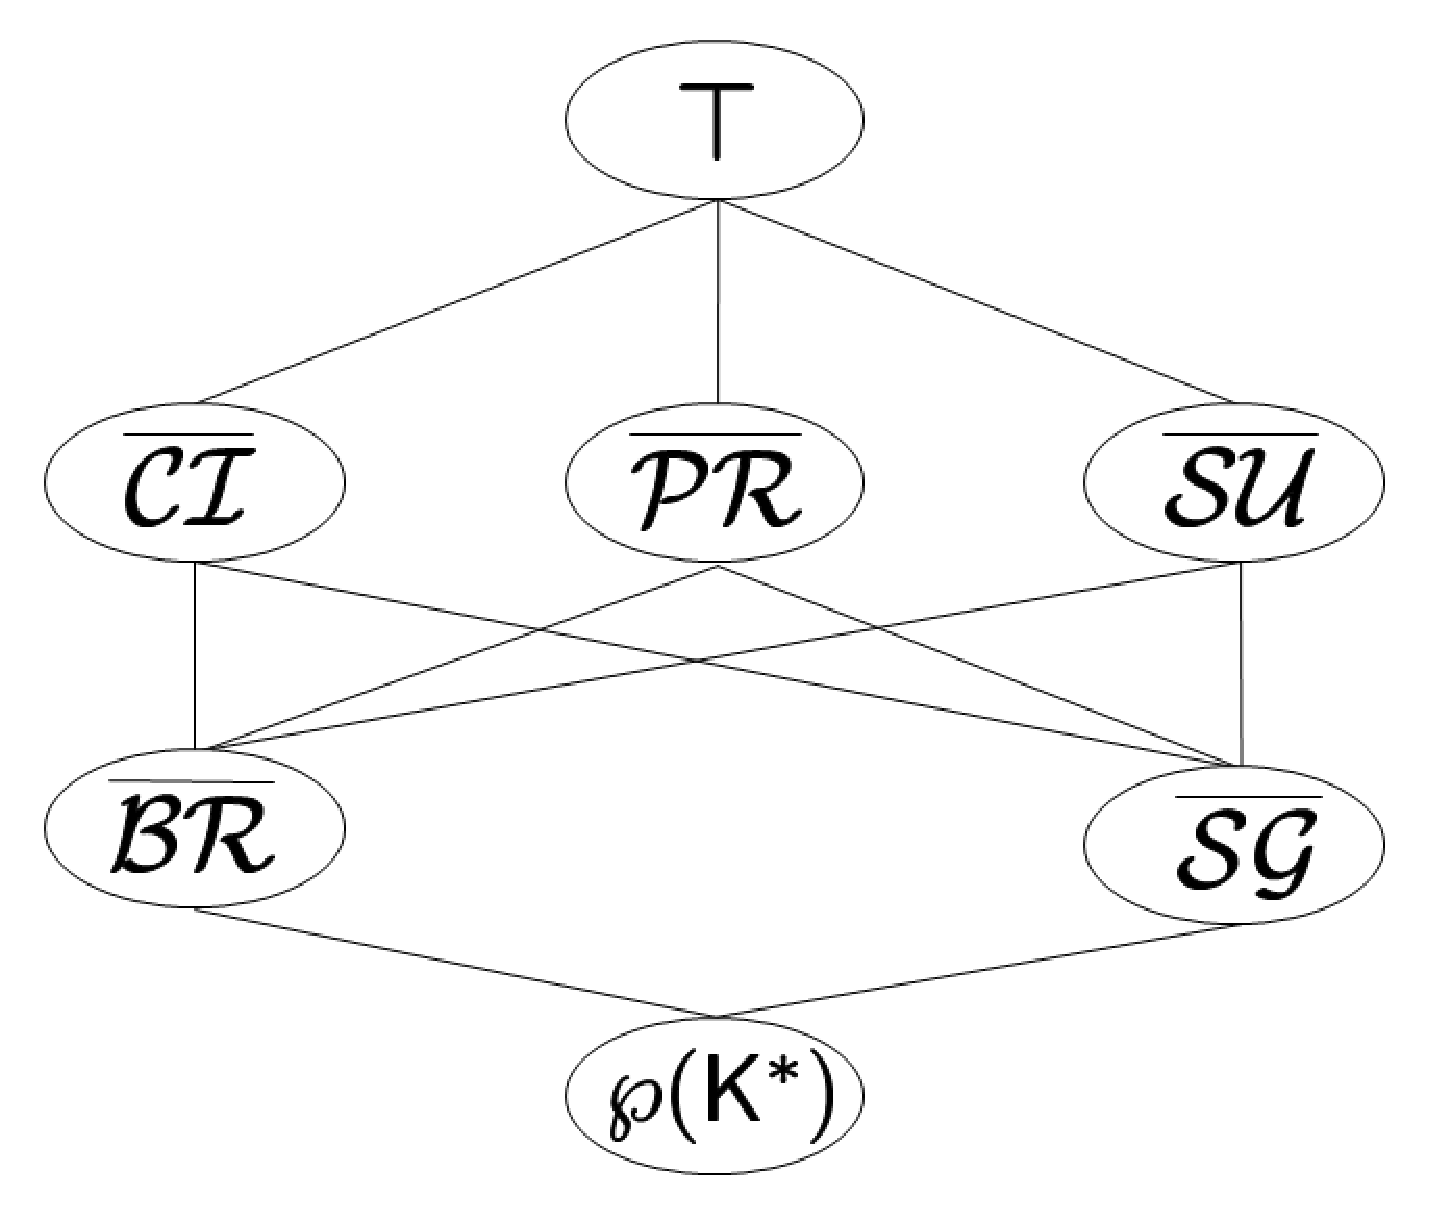
\includegraphics[width=4cm]{domainofdomains.eps}
  \end{center}
\caption{The hierarchy of abstract domains}
\label{fig:domainlattice}
\vspace{-10pt}
\end{wrapfigure}
With $\abricks$, instead, we can indicate exactly how many times a certain pattern should be repeated (through the range of bricks). 
This makes $\abricks$ more expressive than $\astringgraphs$ in that respect. So, these domains are not directly comparable. 
We obtain the lattice depicted in Figure \ref{fig:domainlattice}, where the upper domains are more approximated. We denote by $\top$ the abstract domain that does not track any information about string values, and by $\parts{\sequence{\alphabet}}$ the (na\"ive and uncomputable) domain that tracks all the possible strings values we can have.

In conclusion, the first three domains ($\acharsinc$, $\aprefix$, $\asuffix$) are not so precise but the complexity is kept linear, whereas the other domains ($\abricks$ and $\astringgraphs$) are more demanding (though in the practice complexity is still kept polynomial) but also more precise.
 

\section{Related Work}
\label{sect:relatedwork}
The static analysis of strings was addressed in various directions.

Kim and Choe \cite{KC11} introduced recently an approach based on abstract interpretation. They abstract strings with pushdown automata (PDA). The result of the analysis is compared with a grammar to determine if all the strings generated by the PDA belong to the grammar. This approach has a fixed precision, and in the worst case (not often encountered in practice) it has exponential complexity.

Hosoya and Pierce \cite{HOS03} used tree automata to verify dynamically generated XML documents. The regular expression types of this approach recall our $\abricks$ domain, while the tree automata recall our $\astringgraphs$ domain. However, they are focused on building XML documents, while our focus is on collecting possible values of generic string variables. In addition, they require to manually annotate the code through types while our approach is completely automatic.

A more recent work was developed by Yu \emph{et al.} \cite{YU08}. It presented an automata-based approach for the verification of string operations in PHP programs. The information tracked by this analysis is fixed, and it is specific for PHP programs.

Tabuchi \emph{et al.} \cite{TAB02} presented a type system based on regular expressions. It is focused on a $\lambda$-calculus supporting concatenation, and pattern matching. Some type annotation is required when dealing with recursive function.

Thiemann \cite{THI05} introduced a type system for string analysis based on context-free grammars. Their analysis is more precise than those based on regular expressions, but the only supported string operator is concatenation, and the analysis is tuned at a fixed level of precision. 

Context-free grammars are also the basis of the analysis of Christensen \emph{et al.} \cite{CHR03}. This analysis is tuned at a fixed level of abstraction. In the second running example of this paper, $\astringgraphs$ domain reaches a better precision than theirs.

Minamide \cite{MIN05} presented an analysis to statically check some properties of Web pages generated dynamically by a server-side program. This work is specific for HTML pages, while we do not need to know the reference grammar \textit{a priori}. Also in this case, $\astringgraphs$ obtain a better precision on the loop example.

Doh \emph{et al.} \cite{DOH09} proposed a technique called ``abstract parsing": it combines LR(k)-parsing technology and data-flow analysis to analyse  dynamically generated documents. Their technique is quite precise, but the level of abstraction is fixed, and it cannot be tuned at different levels of precision and efficiency.

Given this context, our work is the first one that (i) is a generic, flexible, and extensible approach to the analysis of string values, and (ii) can be tuned at different levels of precision and efficiency.

 
 
\section{Conclusion and Future Work}
\label{sect:conclusion}
In this paper we introduced a new framework for the static analysis of string values, and four different abstract domains. We chose some string operators on which we focused our approach defining the concrete and the abstract semantics.

\noindent \textbf{Future work} We are working on the implementation of our approach in $\Sample$ (Static Analyzer of Multiple Programming LanguagEs) \cite{FER10}. We plan to apply our analysis to some case studies to study the precision of our analysis. In order to check the scalability and performances of our approach, we plan to apply our analysis to some Scala standard libraries. Some preliminary experimental results point out that $\acharsinc$ and $\aprefix \times \asuffix$ are quite efficient, $\abricks$ is slower but still fast, while $\astringgraphs$'s performances seem to be still critical.
\subsubsection*{Acknowledgments.} Work partially supported by RAS project \textquotedblleft TESLA - Tecniche di enforcement per la sicurezza dei linguaggi e delle applicazioni\textquotedblright, and by SNF project \textquotedblleft Verification-Driven Inference of Contracts\textquotedblright.

\bibliographystyle{abbrv}
\bibliography{bibliografia}

\end{document}
